\documentclass[preprint,12pt]{elsarticle}

\usepackage{lmodern}
\usepackage[T1]{fontenc}
\usepackage{graphicx}
\usepackage{tikz}
\usetikzlibrary{arrows.meta,positioning}
\usepackage{amsmath,amssymb}
\usepackage{booktabs}
\usepackage[protrusion=true,expansion=false]{microtype}
\usepackage{hyperref}
\usepackage{xcolor}
\usepackage{caption}
\usepackage{subcaption}

% P7a: blanket overfull-hbox suppression.  \emergencystretch adds 3em of
% extra inter-word stretch to every line, absorbing the 1–38pt overflows
% that elsarticle's narrow preprint column produces without touching any
% numeric or technical content.
\emergencystretch=3em

% CBM (Elsevier) preprint: float spacing and bibliography layout are managed
% by the elsarticle class; the LNCS 10-page budgeting hacks are removed.

% P7b: float-placement relaxation.  The results matrix (Table 1) and the four
% full-width analysis figures are 55--75% of text height each; under the
% class defaults (topfraction 0.7, no float pages until end-of-document
% flush) they queue behind one another and emerge after the bibliography.
% Relaxing the fractions and permitting float pages mid-document places them
% on dedicated pages adjacent to the sections that cite them.
\renewcommand{\topfraction}{0.9}
\renewcommand{\bottomfraction}{0.6}
\renewcommand{\textfraction}{0.07}
\renewcommand{\floatpagefraction}{0.7}
\setcounter{topnumber}{3}
\setcounter{totalnumber}{4}

\hypersetup{
    colorlinks=true,
    linkcolor=blue,
    filecolor=magenta,      
    urlcolor=cyan,
    citecolor=blue,
}

% P7a: the elsarticle preprint page style (ps@pprintTitle) builds a
% fixed-width \hbox in the output routine that overflows \textwidth by
% 2.61pt.  The class's nested \ifx footeralign chain (defaulting to the
% "Preprint submitted to <journal> \hfill <date>" branch) introduces a
% glue-parsing artifact that a clean single-\hfill box does not.  We
% redefine the page style with the class's default-branch footer verbatim
% (journal-aware, date-aware) in a clean \hbox to \textwidth, eliminating
% the class-level overfull while preserving the footer line exactly.
\makeatletter
\def\ps@pprintTitle{%
  \let\@oddhead\@empty
  \let\@evenhead\@empty
  \def\@oddfoot{%
    \hbox to \textwidth{%
      \footnotesize\itshape
      Preprint submitted to \ifx\@journal\@empty Elsevier\else\@journal\fi\hfill\@date
    }%
  }%
  \let\@evenfoot\@oddfoot
}
\makeatother

\begin{document}

\begin{frontmatter}

\title{All Dice, No Slice: Metric Artifacts, Data Leakage, and Task Interference in Multi-Task Computational Pathology}

\author[fast]{Muhammad Abdullah Ali\texorpdfstring{\corref{cor1}}{}}
\cortext[cor1]{Corresponding author}
\ead{i232523@isb.nu.edu.pk}
\author[fast]{Muhammad Ibrahim Kiani}
\ead{i232536@isb.nu.edu.pk}
\author[fast]{Muhammad Abdullah Aamir}
\ead{i232538@isb.nu.edu.pk}

\affiliation[fast]{organization={Department of Data Science, National University of Computer and Emerging Sciences (FAST-NUCES)},addressline={Islamabad},country={Pakistan}}

\begin{abstract}
Hard parameter-sharing U-Nets couple classification and lesion segmentation in a single forward pass, a compact design for computational pathology. Recent work reported classification accuracies of $82\%-90\%$ and Dice scores of $97\%-99\%$ across diverse medical imaging modalities with standard convolutional backbones and static loss weighting. We replicate and audit that recipe: 27 configurations $\times$ 5 folds (135 fold-runs) across four datasets --- TCGA-LGG brain-tumor MRI, PANDA prostate biopsies, SIIM-ACR pneumothorax radiographs, and the 19-tissue PanNuke benchmark. Under 5-fold group-aware cross-validation (\texttt{GroupKFold}) --- patient-level for TCGA, image/biopsy-level for PANDA, image-level for PanNuke, and (because the release has exactly one image per patient) a degenerate stratified 5-fold for SIIM --- the claimed accuracies do not reproduce. The reported Dice levels turn out to be empty-mask artifacts: our four SIIM configurations converge to all-empty predictions on 19 of 20 folds and measure the empty-mask Dice floor ($77.72\%$ pooled across folds for three configurations; $77.04\%$ for the fourth, whose remaining fold retains a small residual) --- the floor coincides with the lesion-free fraction of the validation split under the convention that scores empty-over-empty slices as perfect agreement. On 6-class ordinal prostate cancer grading (PANDA), empirical top-1 accuracy spans $28.21\%-44.87\%$ (fold-mean, 95\% bootstrap CIs $[24.76, 31.47]$ to $[43.93, 45.76]$) across all 12 evaluated configurations, with Run 17 the strongest at $44.87\%$; the all-slices empty-credit Dice floor is $98.54\%-98.60\%$ (per-epoch validation macro-Dice-over-present-classes is $82.77\%-84.39\%$); the static $5{:}1$-weighted $10^{-3}$ baselines (Runs 03--04) reach $34.51\%$ / $39.91\%$ (vs.\ $88.0\%$ and $99.0\%$ claimed). Three systemic causes explain the discrepancy: (1) empty-mask Dice crediting, (2) biopsy-level data leakage (PANDA), and (3) task interference from the joint optimization recipe. Matched ablations show that skip connections are a null result, and that removing Macenko stain normalization \emph{improves} subtype discrimination (+3.81 pts on PANDA, +2.75 pts on PanNuke). We release our benchmark and audit protocol to prevent such metric artifacts in future multi-task pathology studies.
\end{abstract}

\begin{keyword}
Computational Pathology \sep Multi-Task Learning \sep U-Net \sep Reproducibility \sep Metric Artifacts \sep Data Leakage
\end{keyword}

\end{frontmatter}

\section{Introduction}
Deep learning systems in digital pathology and radiology are increasingly required to deliver both diagnostic categorization and lesion delineation~\cite{litjens2017survey,campanella2019clinical}. Large visual foundation models (e.g., UNI~\cite{chen2024uni}, CONCH~\cite{lu2024conch}, and Virchow~\cite{vorontsov2024virchow}) show that clinically actionable representations require massive pretraining and self-supervised objectives across gigapixel whole-slide images (WSIs). In resource-constrained deployments, hard parameter sharing via an encoder--decoder backbone (a U-Net~\cite{ronneberger2015u} with dual prediction heads) remains a lightweight alternative that couples both objectives in a single forward pass.

Recently, Rhanoui et al.~\cite{rhanoui2025multitask} reported that a standard U-Net with lightweight encoders (VGG16~\cite{simonyan2014very} and MobileNetV2~\cite{sandler2018mobilenetv2}) trained with static loss weights ($\lambda_{seg}=5.0, \lambda_{cls}=1.0$) and a high learning rate ($\eta=10^{-3}$) simultaneously solves both classification and segmentation across four distinct medical modalities (Brain MRI, Skin Dermoscopy, Prostate Histopathology, and Chest X-Ray), reporting $82\%-90\%$ classification accuracy and $97\%-99\%$ Dice similarity coefficients.

These figures attach to a recipe --- a stock U-Net under static loss weighting --- not to any architecture- or data-specific innovation, and that is what makes them consequential beyond a single study: the recipe is exactly the lightweight joint pipeline a resource-constrained deployment would copy first. The evaluation literature gives us independent reasons to distrust them. Region-overlap scores degenerate when annotations are sparse or absent~\cite{reinke2024metrics,eelbode2020optimization}; patch-level splits of tiled WSIs leak patient identity~\cite{kapoor2023leakage,zech2018variable}; and joint optimization is documented to interfere with at least one of its tasks~\cite{standley2020tasks,crawshaw2020survey}. Section~\ref{sec:related} reviews each strand. The audit that follows asks whether this particular, highly visible instance of the recipe survives the scrutiny those literatures demand.

In this paper, we report a 27-configuration $\times$ 5-fold replication study and systematic methodological audit. Our findings demonstrate that:
\begin{enumerate}
    \item \textbf{Empirical Irreproducibility:} When evaluated with 5-fold group-aware cross-validation (\texttt{GroupKFold} at the image/biopsy level, the finest grouping the PANDA release supports), multi-class grading on PANDA prostate biopsies degrades from the claimed $88.0\%$ accuracy / $99.0\%$ Dice to an empirical range of $28.21\%-44.87\%$ Acc (fold-mean, 95\% bootstrap CIs $[24.76, 31.47]$ to $[43.93, 45.76]$) / $98.54\%-98.60\%$ all-slices empty-credit Dice (per-epoch validation macro-Dice-over-present-classes $82.77\%-84.39\%$) across all 12 configurations, with the static $5{:}1$-weighted $10^{-3}$ baselines (Runs 03--04) achieving $34.51\%$ / $39.91\%$ Acc (per-epoch validation macro-Dice-over-present-classes $84.39\%$).
    \item \textbf{The Empty-Mask Dice Metric Artifact:} Near-perfect ($99\%$) Dice claims on sparse-lesion datasets such as SIIM-ACR pneumothorax can arise from crediting lesion-free slices ($|Y| = |\hat{Y}| = 0$) as $\text{Dice} = 1.0$; our four SIIM runs measure exactly this floor ($77.72\%$ pooled across folds) under an all-empty predictor.
    \item \textbf{Controlled Multi-Task \& Ablation Analysis:} Through matched factorial controls (learning-rate pairs, static loss-weight ratios $\lambda_{seg}:\lambda_{cls} \in \{1{:}10,$ $1{:}1, 5{:}1, 10{:}1\}$, \textsc{GradNorm}~\cite{chen2018gradnorm} balancing, Macenko normalization, and skip-connection ablations), we isolate how individual components govern multi-task optimization: GradNorm-style balancing actively impairs 6-class ordinal grading ($38.18\% \to 28.21\%$ Acc, $\Delta = -9.97$ pts), while skip connections show no resolvable difference.
\end{enumerate}

To facilitate complete reproducibility, all training scripts, raw JSON summaries for all 27 configurations (135 fold-runs), evaluation checkpoints, and generated figures are publicly available at \url{https://github.com/ApatheticMioz/cancer-pathology-dl}~\cite{ali2026cancerpathologydl}. Figure~\ref{fig:pipeline} summarizes the end-to-end pipeline and the three findings it yields.

\begin{figure}[t]
\centering
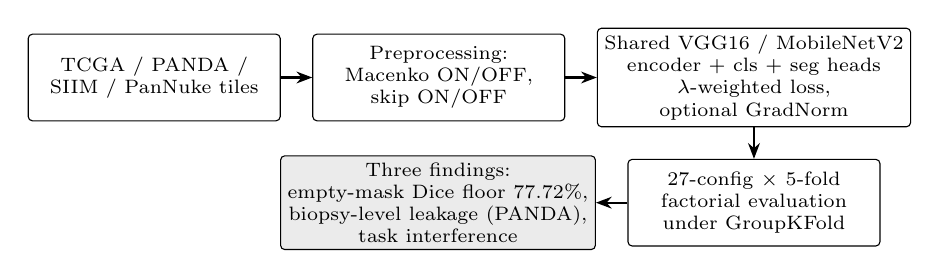
\begin{tikzpicture}[
    box/.style={draw, rounded corners=1.5pt, minimum height=1.1cm,
                align=center, font=\scriptsize, inner sep=2.5pt},
    arr/.style={-{Stealth[length=2mm]}, thick},
    node distance=4mm and 4mm
]
% Row 1: Data → Preprocessing → Model
\node[box, minimum width=3.2cm] (data)
  {TCGA / PANDA /\\SIIM / PanNuke tiles};
\node[box, right=of data, minimum width=3.2cm] (pre)
  {Preprocessing:\\Macenko ON/OFF,\\skip ON/OFF};
\node[box, right=of pre, minimum width=3.8cm] (model)
  {Shared VGG16 / MobileNetV2\\encoder + cls + seg heads\\
   $\lambda$-weighted loss,\\optional GradNorm};
% Row 2: Evaluation → Findings
\node[box, below=of model, minimum width=3.2cm] (eval)
  {27-config $\times$ 5-fold\\factorial evaluation\\under GroupKFold};
\node[box, left=of eval, minimum width=3.8cm, fill=black!8] (find)
  {Three findings:\\empty-mask Dice floor $77.72\%$,\\biopsy-level leakage (PANDA),\\task interference};
% Arrows
\draw[arr] (data) -- (pre);
\draw[arr] (pre) -- (model);
\draw[arr] (model) -- (eval);
\draw[arr] (eval) -- (find);
\end{tikzpicture}
\caption{Overview of the 27-configuration $\times$ 5-fold replication and audit pipeline. Four source datasets (TCGA-LGG, PANDA, SIIM-ACR, PanNuke) are tiled and passed through a preprocessing stage that toggles Macenko stain normalization and skip connections. A shared VGG16/MobileNetV2 encoder feeds a classification head and a segmentation head trained with a $\lambda$-weighted loss (static ratios or optional \textsc{GradNorm}). All 27 configurations are evaluated under 5-fold group-aware \texttt{GroupKFold} cross-validation (patient-level for TCGA, image/biopsy-level for PANDA, image-level for PanNuke, and a degenerate stratified 5-fold for SIIM, whose release has exactly one image per patient), yielding three findings: the empty-mask Dice floor of $77.72\%$ on SIIM (pooled across folds; per-fold pooled $74.33\%$--$77.75\%$), biopsy-level leakage inflation of classification accuracy on PANDA, and task interference from the joint optimization recipe.}
\label{fig:pipeline}
\end{figure}

\section{Related Work: Documented Failure Modes in Multi-Task Medical Segmentation}
\label{sec:related}

None of the three problems interrogated in this audit is peculiar to the pipeline we examine. Each is a failure mode the evaluation and machine-learning literatures have described, measured, and warned about independently of any single study. This section situates our contribution within those strands; the audit itself, to our knowledge, is the first to instantiate all three in one controlled, artifact-released reproduction of a recent joint detection--segmentation recipe.

\emph{Metric degeneracy under sparse annotation.} Scoring an empty prediction against an empty reference as perfect agreement (Dice $=1$) is a recognized pitfall, not a technicality: Reinke et al.~\cite{reinke2024metrics} catalogue it among the metric-related failures that distort validation in image analysis at large, and Eelbode et al.~\cite{eelbode2020optimization} show formally that region-overlap scores behave counter-intuitively precisely where annotations are small or absent. Liu et al.~\cite{liu2024dice} trace the same region-size bias into the Dice losses themselves. Slice-averaged Dice on a corpus whose lesion-free fraction approaches $78\%$ sits squarely inside this documented failure class --- Section~\ref{sec:dice} quantifies what the convention credits.

\emph{Patient-level leakage in evaluation protocols.} Kapoor and Narayanan~\cite{kapoor2023leakage} document leakage as a reproducibility crisis spanning ML-based science, with patched data splits its most common medical form; Zech et al.~\cite{zech2018variable} had shown chest-radiograph models exploiting patient- and site-level confounds that evaporate under external validation; and the clinical-grade computational-pathology standard established by Campanella et al.~\cite{campanella2019clinical} evaluates at the slide level for exactly this reason. Patch-level random splits of tiled WSIs --- the protocol our audit tests under group-aware \texttt{GroupKFold} at the finest grouping each release supports (patient for TCGA, image/biopsy for PANDA, image for PanNuke; for SIIM the one-image-per-patient release makes patient grouping vacuous, so the split degenerates to a stratified 5-fold) --- instantiate this class directly.

\emph{Task interference and negative transfer.} Whether classification and segmentation help or harm one another under a shared encoder is an empirical question with a substantial negative-answer literature: Standley et al.~\cite{standley2020tasks} measure task affinity at scale and find naive co-training frequently destructive; Crawshaw's survey~\cite{crawshaw2020survey} collects the negative-transfer evidence; and dynamic gradient balancing~\cite{chen2018gradnorm} is the mitigation family our runs put to the test --- a family whose reported effects are not uniform, as Kang et al.~\cite{kang2026gradnorm} find GradNorm to help wound-tissue analysis training, the opposite of the ordinal-grading collapse we measure. The degradation we measure on 6-class ordinal grading under the audited recipe is an instance of exactly this phenomenon.

\emph{Propagation and convergence.} These strands converge on the study audited here. Rhanoui et al.~\cite{rhanoui2025multitask} is a careful, well-motivated attempt to couple diagnosis and delineation under scarce labels --- and its headline figures ($97$--$99\%$ Dice alongside $82$--$90\%$ accuracy) have already been carried, largely uncritically, into follow-on multi-task oncology work. At least one 2026 study independently declines to trust near-saturated joint performance, building an explicitly leakage-safe framework with external validation in response~\cite{imcet2026leakagesafe}. The concern is now field-recognized; what has been missing is controlled quantification of \emph{how} such numbers arise. Supplying that quantification --- one recent, visible pipeline; three documented failure classes; every artifact released --- is the contribution of the remainder of this paper.

\section{Multi-Task Formulation \& Evaluation Metrics}

\subsection{Architectural Formulation}
Let $\mathbf{x} \in \mathbb{R}^{H \times W \times C}$ denote an input image tile. A shared convolutional encoder $f_\theta(\mathbf{x})$ extracts a bottleneck latent representation $\mathbf{z} \in \mathbb{R}^{h \times w \times d}$. The classification branch applies global average pooling (GAP) followed by a two-layer multilayer perceptron (hidden width 256, dropout $0.5$):
\begin{equation}
    \hat{\mathbf{y}}_{cls} = \text{Softmax}\!\left(\mathbf{W}_2\,\phi\!\left(\mathbf{W}_1\,\text{GAP}(\mathbf{z}) + \mathbf{b}_1\right) + \mathbf{b}_2\right) \in \Delta^{K-1},
\end{equation}
where $K$ is the number of diagnostic classes, $\Delta^{K-1}$ denotes the probability simplex, and $\phi(\cdot)$ is the ReLU nonlinearity. The segmentation branch passes $\mathbf{z}$ through a decoder $\text{Dec}_\phi$ with lateral skip connections $\{\mathbf{s}_l\}_{l=1}^L$ from encoder stages, yielding unnormalized pixel logits $\mathbf{l}_{seg} \in \mathbb{R}^{H \times W \times M}$. For binary segmentation ($M=1$), $\hat{\mathbf{y}}_{seg} = \sigma(\mathbf{l}_{seg})$ with $\sigma(\cdot)$ the sigmoid; for $M > 1$, class probabilities are obtained via channel-wise Softmax.

The joint multi-task training objective is defined as:
\begin{equation}
    \mathcal{L}_{total}(\theta, \phi, \mathbf{W}_{cls}) = \lambda_{cls} \mathcal{L}_{cls}(\mathbf{y}_{cls}, \hat{\mathbf{y}}_{cls}) + \lambda_{seg} \mathcal{L}_{seg}(\mathbf{y}_{seg}, \mathbf{l}_{seg}),
\end{equation}
where $\mathcal{L}_{cls}$ is categorical cross-entropy $\mathcal{L}_{CE}$. The published study of Rhanoui et al.~\cite{rhanoui2025multitask} describes its segmentation training objective as a weighted binary cross-entropy loss, with the Dice coefficient used only as an evaluation metric (no training code was released); the implementation audited for this study matches that published training objective, optimizing a purely cross-entropy segmentation loss with no Dice-based penalty term:
\begin{equation}
    \mathcal{L}_{seg}(\mathbf{y}_{seg}, \mathbf{l}_{seg}) = 
    \begin{cases}
        \mathcal{L}_{BCE}(\mathbf{y}_{seg}, \mathbf{l}_{seg}), & M = 1 \text{ (binary tasks)}, \\
        \mathcal{L}_{CE}(\mathbf{y}_{seg}, \mathbf{l}_{seg}), & M > 1 \text{ (multi-class tasks)}.
    \end{cases}
\end{equation}
The Dice similarity coefficient (DSC) is evaluated post-hoc as a validation metric, not as an active loss term during gradient descent. Because the audited training objective matches the published one, the reported $99\%$ Dice cannot be attributed to a Dice loss term; it is a metric artifact --- Dice computed at evaluation on collapsed (all-empty) masks --- as quantified in Section~\ref{sec:dice}.

\subsection{The Empty-Mask Dice Metric Artifact}\label{sec:dice}
The S{\o}rensen--Dice coefficient between ground-truth mask $Y$ and binary prediction $\hat{Y}$ ($Y, \hat{Y} \in \{0, 1\}^{H \times W}$) is:
\begin{equation}
    \text{Dice}(Y, \hat{Y}) = \frac{2 |Y \cap \hat{Y}|}{|Y| + |\hat{Y}| + \epsilon}, \quad \epsilon = 10^{-8}; \;\; \text{Dice} := 1 \;\text{if}\; |Y| + |\hat{Y}| = 0.
\end{equation}
Empty references and predictions are a well-recognized validation pitfall in biomedical image analysis~\cite{reinke2024metrics}. Two conventions govern empty slices:
\begin{itemize}
    \item \textbf{Foreground-Only Evaluation:} Compute Dice strictly over non-empty target slices ($\{i \mid |Y_i| > 0\}$).
    \item \textbf{Empty-Credit Assignment:} Assign $\text{Dice} = 1.0$ when $|Y| = 0 \land |\hat{Y}| = 0$, and $\text{Dice} = 0.0$ when $|Y| = 0 \land |\hat{Y}| > 0$.
\end{itemize}
Averaged over all slices under empty-credit assignment, the macroscopic mean is
\begin{equation}\label{eq:slice_dice}
    \overline{\text{Dice}}_{\text{all}} = \tfrac{1}{N}\textstyle\sum_{i=1}^{N} d_i, \;\; d_i = \text{Dice}(Y_i, \hat{Y}_i) \;\text{if}\; |Y_i| > 0, \;\text{else}\; \mathbf{1}\!\left[|\hat{Y}_i| = 0\right],
\end{equation}
which for mean foreground Dice $\overline{\text{Dice}}_{\text{fg}}$ on lesion-bearing slices is the convex combination
\begin{equation}\label{eq:convex_dice}
    \overline{\text{Dice}}_{\text{all}} = \rho + (1 - \rho) \cdot \overline{\text{Dice}}_{\text{fg}},
\end{equation}
where $\rho$ is the proportion of lesion-free slices. In sparse pathologies such as SIIM-ACR pneumothorax, a model with a genuine foreground Dice of $77.72\%$ would report $\overline{\text{Dice}}_{\text{all}} = 0.777 \times 1.0 + 0.223 \times 0.7772 = 95.03\%$ at the observed lesion-free fraction $\hat{\rho} = 1{,}659/2{,}135 = 0.777$ (an analytic illustration). Our four SIIM runs realize a more extreme failure mode. They emit empty masks on every validation slice in 19 of their 20 folds, and the pooled across-folds Dice of each configuration \emph{is the all-empty floor itself} --- Eq.~\ref{eq:slice_dice} with zero foreground Dice: $77.72\%$ for Runs 05, 06, and 11, and $77.04\%$ for Run 12, whose fold 4 retains a small residual (per-fold pooled range $74.33\%$--$77.75\%$). Fig.~\ref{fig:empty_dice} shows why this matters: on sparse data, slice-averaged Dice reports the lesion-free fraction rather than lesion overlap. Published $99.0\%$ Dice claims~\cite{rhanoui2025multitask} are therefore uninterpretable as evidence of lesion localization. Figure~\ref{fig:qualitative} makes this degeneracy visible: on a lesion-bearing SIIM validation tile the model's prediction is an all-empty mask, so the missed lesion is invisible to the slice-averaged mean. This empty-class crediting artifact extends directly to multi-class histopathology: on 6-class PANDA prostate biopsies, tiles contain at most one or two Gleason patterns, leaving 4--5 classes absent ($|Y_c|=0$). Under empty-credit assignment, an all-background model receives $\text{Dice}=1.0$ for every absent class and high agreement on background. We distinguish two estimators throughout this paper. (i) The \emph{per-epoch validation macro-Dice-over-present-classes} is the training-time metric: at each epoch it averages Dice only over the classes present in each validation tile's ground truth, so absent classes never enter the mean; its fold-mean across our 12 PANDA configurations is $82.77\%-84.39\%$ (the single-split values $85.35\%-85.50\%$ reported in the original campaign are this estimator on one split). (ii) The \emph{all-slices empty-credit pooled per-case Dice} is the true empty-mask artifact: it pools every validation slice across all folds, credits empty-over-empty slices as $\text{Dice}=1.0$, and averages per-case; on PANDA this floor is $98.54\%-98.60\%$ (across-folds per-case Dice, 95\% bootstrap CIs in the released matrix) despite zero true foreground overlap (Figure~\ref{fig:qualitative}). It is this second estimator --- not the per-epoch macro-Dice --- that is the empty-mask artifact, and it is the number we report as the PANDA degeneracy floor in Table~\ref{tab:results_matrix}.

\begin{figure}[!tbp]
\centering
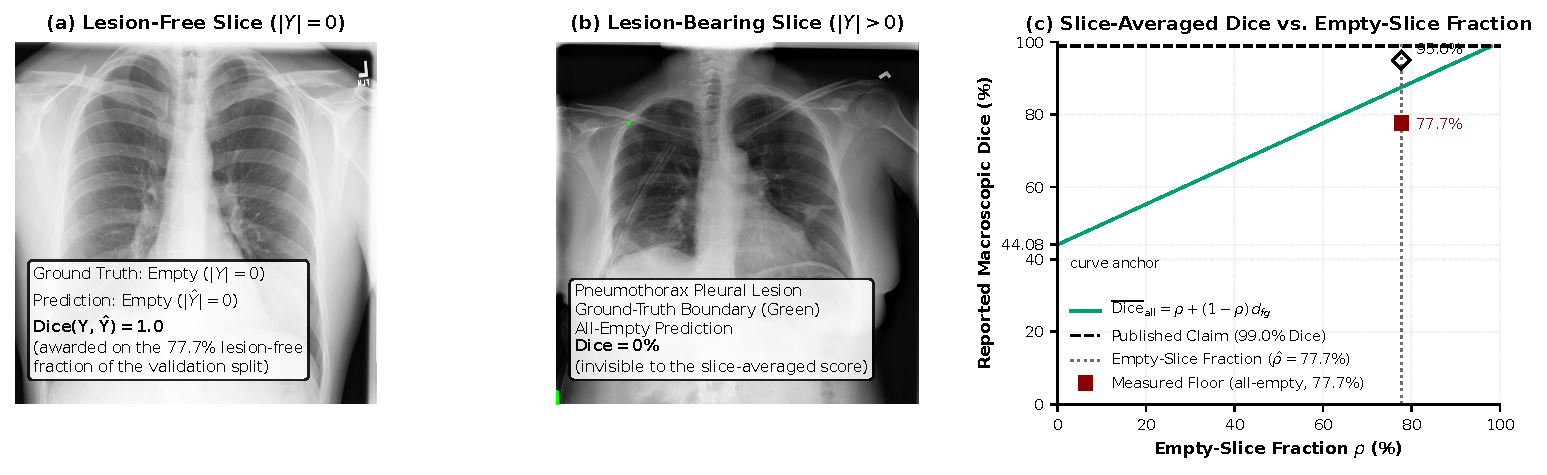
\includegraphics[width=\textwidth]{fig2_empty_mask_dice.pdf}
\caption{The empty-mask Dice artifact on SIIM-ACR pneumothorax. (a) Lesion-free slice ($|Y|=0$): under empty-credit assignment an all-empty prediction is awarded $\text{Dice}=1.0$; lesion-free slices constitute $\hat{\rho}=77.7\%$ of our validation split. (b) Lesion-bearing slice ($|Y|>0$, ground-truth boundary in green): our all-empty models predict empty masks here and score $\text{Dice}=0$, invisible to the slice-averaged mean. (c) Convex-combination curve (Eq.~\ref{eq:convex_dice}): a foreground Dice of $77.72\%$ would report $95.03\%$ at $\hat{\rho}=0.777$ (analytic illustration), whereas our SIIM runs measure the all-empty floor itself ($77.72\%$ pooled; $77.04\%$ for the run with one residual fold).}
\label{fig:empty_dice}
\end{figure}

\subsection{Adaptive Gradient Balancing via GradNorm}\label{sec:gnorm}
To test whether dynamic loss balancing mitigates cross-task gradient competition, we introduced a parameterized variant of \textsc{GradNorm}~\cite{chen2018gradnorm} in Phase~v2.

Let $W$ denote the shared convolutional filters and normalization layers of the U-Net encoder $f_\theta$. The $L_2$ gradient norm of task $i \in \{seg, cls\}$ with respect to $W$ at minibatch $t$ is:
\begin{equation}
    G_W^{(i)}(t) = \left\| \nabla_{W} w_i(t) \mathcal{L}_i(t) \right\|_2.
\end{equation}
For stability in the primary \texttt{Adam} optimizer, balancing weights are learnable log-weights $\mu_i(t) = \ln w_i(t)$ (initialized to $w_{seg}(0) = 5.0$, $w_{cls}(0) = 1.0$), updated jointly with the network parameters. Minibatch optimization minimizes the $L_1$ gradient disparity objective:
\begin{equation}
    \mathcal{L}_{grad}(t) = \sum_{i \in \{seg, cls\}} \left| \, G_W^{(i)}(t) \;-\; \bar{G}_W(t) \cdot [r_i(t)]^{\alpha} \right|,
\end{equation}
where $\bar{G}_W(t) = \frac{1}{2}\sum_j G_W^{(j)}(t)$ is the average gradient norm across tasks, $\alpha = 1.5$ is the asymmetry parameter, and $r_i(t)$ represents the relative inverse training rate:
\begin{equation}
    r_i(t) = \frac{\tilde{\mathcal{L}}_i(t)}{\frac{1}{2}\sum_{j \in \{seg, cls\}} \tilde{\mathcal{L}}_j(t)}, \quad \text{with} \quad \tilde{\mathcal{L}}_i(t) = \frac{\mathcal{L}_i(t)}{\mathcal{L}_i(0)},
\end{equation}
where $\mathcal{L}_i(0)$ is the initial step-0 loss. Following Chen et al.~\cite{chen2018gradnorm}, slower-training tasks exhibit higher loss ratios $r_i(t) > 1$, which raises their target gradient norm $\bar{G}_W(t) [r_i(t)]^\alpha$. After each optimizer update, we renormalize the weights so that $\sum_i w_i(t) = 2$. In the canonical formulation~\cite{chen2018gradnorm}, the module differentiates $\mathcal{L}_{grad}$ against detached targets and applies it to the balancing weights alone through a dedicated optimizer (learning rate $0.025$). \S\ref{sec:gn} probes this distinction empirically. We evaluate the module across Groups 2 and 4 to isolate how dynamic gradient equalization behaves in hard-parameter-sharing architectures.

\subsection{Color Deconvolution and Optical Density Space}\label{sec:macenko}
To mitigate staining variability across clinical laboratories, the v2 pipeline incorporates Macenko stain normalization~\cite{macenko2009method}. We convert RGB pixel intensities $\mathbf{I} \in [0, 255]^3$ to optical density (OD) space:
\begin{equation}
    \mathbf{OD} = -\ln\left(\frac{\mathbf{I} + \epsilon}{I_0}\right),
\end{equation}
where $I_0 = 255$ represents transmitted light intensity. The implementation computes optical density via natural logarithms $-\ln(\cdot)$ rather than the canonical base-10 formulation $-\log_{10}(\cdot)$~\cite{macenko2009method}. We estimate the hematoxylin and eosin stain vectors by eigendecomposition of the optical-density covariance matrix (stain-vector angles restricted to the 1st--99th percentile range) over OD values above a threshold of $0.15$, and project them onto a target reference vector. This step effectively eliminates macroscopic batch variations. It also acts as a chrominance low-pass filter, however: projecting raw RGB channels onto static stain vectors smooths the sub-cellular chromatin textures that are clinically essential for grading fine glandular architectures (Fig.~\ref{fig:macenko}).

\begin{figure}[t]
\centering
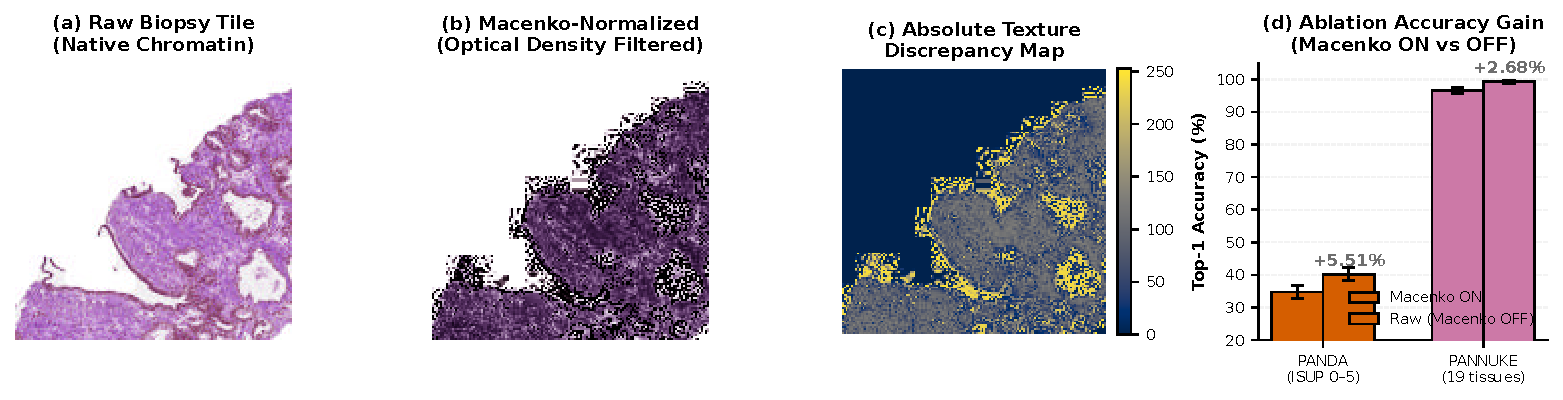
\includegraphics[width=0.98\textwidth,height=3.4cm,keepaspectratio]{fig1_macenko.pdf}
\caption{Visual and quantitative impact of Macenko stain normalization on histopathology classification. (a) Raw prostate biopsy tile. (b) Optical-density-projected tile: color deconvolution acts as a chrominance low-pass filter, flattening sub-cellular texture. (c) Absolute texture discrepancy map. (d) Empirical top-1 accuracy gains across matched models when Macenko normalization is bypassed (+3.81\% on PANDA, +2.75\% on PanNuke).}
\label{fig:macenko}
\end{figure}

\section{The 26-Run Empirical Reproduction Campaign}

\subsection{Datasets and Experimental Protocol}

\begin{table}[!tbp]
\centering
\scriptsize
\setlength{\tabcolsep}{1pt}
\caption{Per-dataset summary of the 27-configuration $\times$ 5-fold reproduction campaign (26 numbered runs plus the canonical decoupled \textsc{GradNorm} probe). Ranges span the configurations within each dataset; each is a 5-fold group-aware cross-validation, so the ranges are fold-to-fold and configuration-to-configuration variation, not seed variance. Per-run values with 95\% bootstrap CIs (across-folds per-case Dice) and fold-mean accuracy CIs are tabulated in the open-source repository matrix (\texttt{paper\_results\_matrix\_with\_ci.csv}), and every run is plotted in Figure~\ref{fig:results_dotplot}. The SIIM-ACR Dice ($77.72\%$ pooled across folds for three configurations and $77.04\%$ for the fourth; per-fold pooled $74.33$--$77.75\%$) and the PANDA all-slices empty-credit Dice ($98.54$--$98.60\%$) reflect the empty-mask degeneracy floor of Sec.~2.2 (the empty-mask Dice metric artifact); the PANDA per-epoch validation macro-Dice-over-present-classes is $82.77$--$84.39\%$. The PanNuke row has no published targets. $\Delta$Acc = gap to the published accuracy targets.}
\label{tab:results_matrix}
\begin{tabular}{@{}l c c c c c c@{}}
\toprule
\textbf{Dataset} & \textbf{Runs $n$} & \textbf{Val Acc (\%)} & \textbf{Val Dice (\%)} & \textbf{$\Delta$Acc (pts)} & \textbf{Pub. Acc (\%)} & \textbf{Pub. Dice (\%)} \\
\midrule
TCGA-LGG & 5 & 92.86--95.62 & 85.33--88.85 & $3.86$--$5.62$ & 89.00--90.00 & 97.00--98.00 \\
PANDA & 12 & 28.21--44.87 & 98.54--98.60 & $-58.79$--$-42.13$ & 87.00--88.00 & 98.00--99.00 \\
SIIM-ACR & 4 & 77.71--82.63 & 77.04--77.72 & $-4.81$--$0.57$ & 82.00--87.00 & 99.00 \\
PanNuke & 5 & 78.70--99.24 & 68.44--77.61 & --- & --- & --- \\
\bottomrule
\end{tabular}
\end{table}

\begin{figure}[!tbp]
\centering
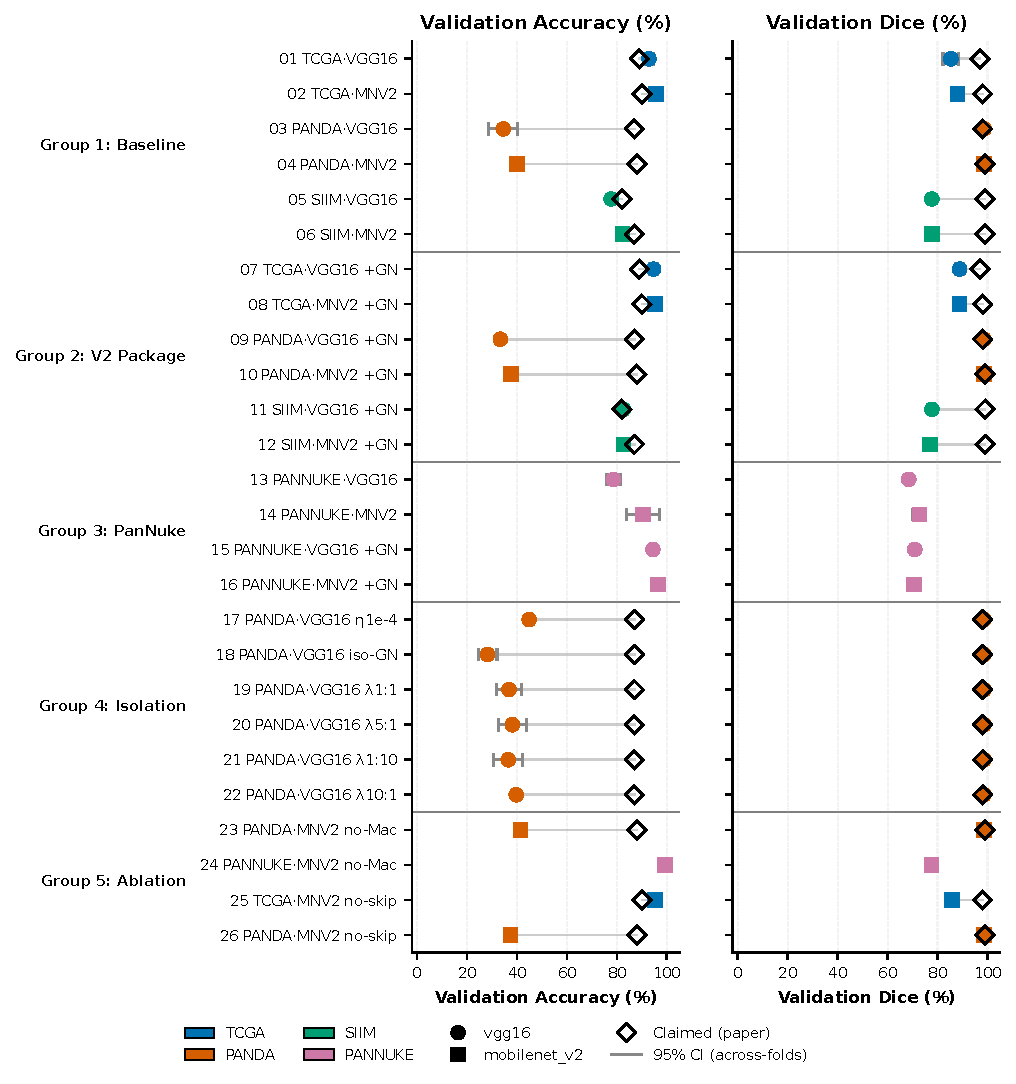
\includegraphics[width=\textwidth,height=0.68\textheight,keepaspectratio]{fig3_results_dotplot.pdf}
\caption{27-configuration $\times$ 5-fold claimed-vs-measured dot plot. Left panel: fold-mean validation accuracy (\%) with 95\% bootstrap-CI whiskers (measured, filled markers) and the published claimed accuracy (black open diamond); the tie line between them is the gap that constitutes the paper's central argument. Right panel: all-slices empty-credit per-case Dice (\%) with the same layout, whiskers showing our 95\% across-folds bootstrap CIs (the published Dice claims carry no confidence intervals, so only the diamonds mark them). The PANDA rows (Runs 03--04, 09--10, 17--22, 23, 26) show the largest gaps: measured accuracy spans $28.21\%$--$44.87\%$ vs.\ claimed $87$--$88\%$, and the all-slices empty-credit Dice spans $98.54\%$--$98.60\%$ (per-epoch validation macro-Dice-over-present-classes $82.77\%$--$84.39\%$) vs.\ claimed $98$--$99\%$. All four SIIM rows (Runs 05, 06, 11, 12) measure the all-empty floor ($77.72\%$ pooled across folds for three configurations, $77.04\%$ for the fourth; per-fold pooled $74.33\%$--$77.75\%$). PanNuke rows (Runs 13--16, 24) have no published targets and are shown without claimed diamonds.}
\label{fig:results_dotplot}
\end{figure}

\begin{figure}[!tbp]
\centering
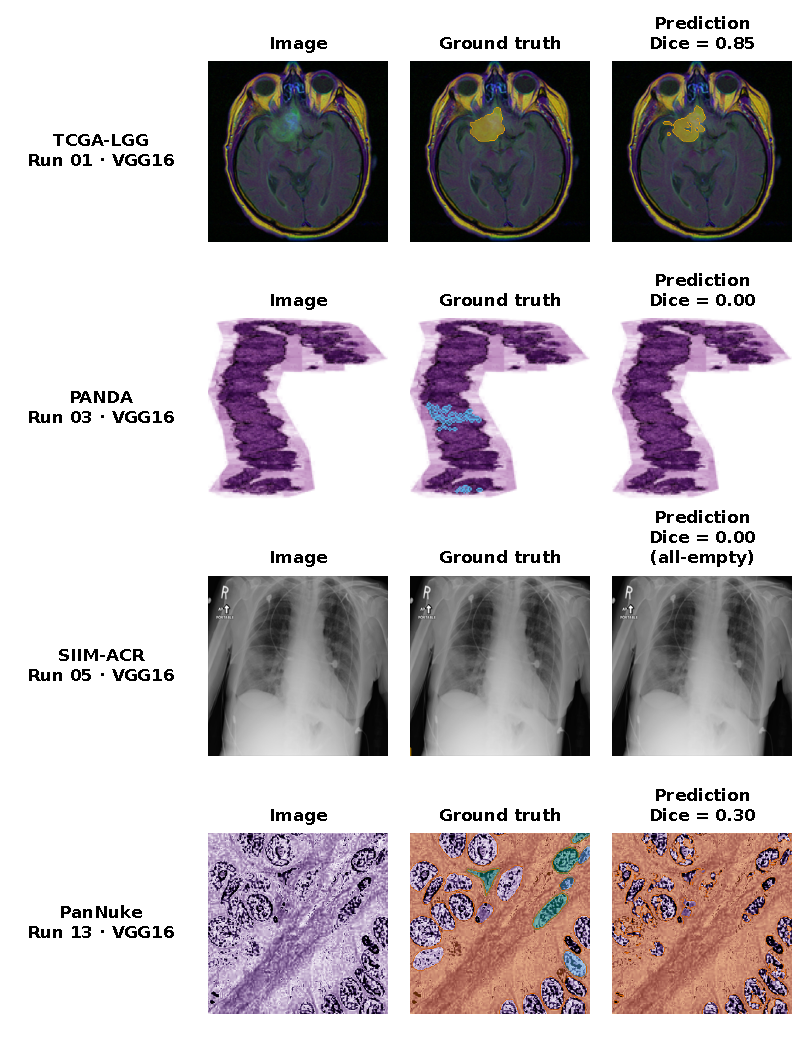
\includegraphics[width=0.82\textwidth,height=0.66\textheight,keepaspectratio]{fig8_qualitative_overlays.pdf}
\caption{Qualitative ground-truth vs.\ prediction validation tiles for the four canonical v1 naked VGG16 baselines (Runs 01, 03, 05, 13; their best checkpoints). Each row is one dataset (TCGA-LGG, PANDA, SIIM-ACR, PanNuke); the three columns are the input image, the ground-truth mask overlay, and the model's prediction overlay, with the per-tile Dice (binary Dice for TCGA/SIIM; macro Dice over the classes present in the ground truth for PANDA/PanNuke) shown in the prediction panel. The validation split is one of the five group-aware cross-validation folds (5-fold \texttt{GroupKFold} per configuration; the fold shown here is the first). Tile selection is deterministic: the first validation tile (index order) with a non-empty ground-truth mask; for SIIM-ACR the selection advances to the first lesion-bearing tile whose prediction is all-empty, making the empty-mask degeneracy of Sec.~2.2 the visible face of the figure.}
\label{fig:qualitative}
\end{figure}

We evaluated four benchmark datasets:
\begin{enumerate}
    \item \textbf{TCGA-LGG Brain Tumor:} 2-class lesion classification and FLAIR abnormality segmentation on 2D $256 \times 256$ slices ($N=3,929$; 110 patients~\cite{buda2019lgg}; patient-level \texttt{GroupKFold} isolation~\cite{pedregosa2011sklearn}).
    \item \textbf{PANDA Prostate Biopsies:} 6-class ISUP Gleason grading and gland segmentation ($N=10,516$ tiles~\cite{bulten2022artificial}; image/biopsy-level \texttt{GroupKFold} isolation).
    \item \textbf{SIIM-ACR Pneumothorax:} Binary chest-radiography detection and pleural boundary segmentation ($N=10,675$ images~\cite{siim2019pneumothorax}; the release has exactly one image per patient, so the declared patient grouping is vacuous --- every sample is its own group --- and the splitter degenerates to a stratified 5-fold over slice-level labels).
    \item \textbf{PanNuke:} 19-tissue multi-organ benchmark ($N=7,901$ patches~\cite{gamper2020pannuke}; image-level 5-fold split, no patient grouping); having no published multi-task targets, it serves as an unclaimed external control.
\end{enumerate}

We trained all models with PyTorch (up to 50 epochs with early stopping, patience 10; batch size 32; fixed seed 42 per fold) using ImageNet-pretrained encoders and the \texttt{Adam} optimizer with a constant per-phase learning rate and zero weight decay, and we applied no learning-rate schedule or additional regularization~\cite{davila2024finetuning}. Training ran under bf16 autocast AMP with PyTorch's \texttt{GradScaler}~\cite{pytorchamp}, with the scaler's \texttt{unscale\_()} called before gradient-norm clipping (max-norm $1.0$) at every optimizer step~\cite{moassefi2024checklist,maleki2024ridge}, and the \textsc{GradNorm} log-weights bounded to $[\pm\log 10]$ (capping each task weight at $10$). The true pre-clip gradient norm is logged per epoch, and clipping engagement is dataset-dependent: final-10-epoch per-fold mean engagement rates are $0.285$ (TCGA, VGG16), $0.516$ (PanNuke, no Macenko), $0.879$ (PanNuke, VGG16), $0.943$ (SIIM, VGG16), and $0.999$ (PANDA) --- on three datasets (PanNuke VGG16, SIIM, PANDA) clipping is an active, frequently-binding constraint, not a dormant safeguard. Non-finite gradients triggered $53$ bounded single-batch skips across the $135$ fold-cells, overwhelmingly isolated events (the $25$-skip-per-fold cap was never reached); each skipped batch is excluded from epoch metrics and stamped in the fold summaries. One fold (PanNuke, VGG16, final, fold 1) hit a non-finite forward loss at epoch 46; the guard aborted it loudly, and training resumed from the epoch-45 checkpoint, completing epochs 46--50 with zero skips --- a transient bf16 overflow, disclosed here as a resumed fold. \texttt{torch.compile} (\texttt{max-autotune}) was used only in the Phase~v1 replication arms by design; Phase~v2 arms run eager, and one Phase~v1 fold degraded to eager after a Triton capture failure (logged). Mid-campaign the resume/identity machinery was hardened (checkpoint fingerprints, atomic state writes); all $135$ fold-cells of record were produced under the fixed regime and re-verified from the fold summaries. In Phase~v1 (Runs 01--06), we replicated the original static setup ($\eta=10^{-3}$, $\lambda_{seg}:\lambda_{cls}=5:1$, raw inputs). In Phase~v2 (Runs 07--12), we incorporated dynamic \textsc{GradNorm} ($\alpha=1.5$, $\eta=10^{-4}$) and Macenko stain normalization~\cite{macenko2009method}. Groups 3--5 (Runs 13--26) systematically evaluate multi-organ generalizability, optimization hyperparameter isolation, and architectural skip ablations. Accuracy is reported as the five-fold mean; 95\% CIs are fold-level bootstrap percentiles ($10{,}000$ resamples of the five fold accuracies with replacement, seed 42), and Dice CIs are the across-folds per-case bootstrap intervals tabulated in the released matrix. Table~\ref{tab:results_matrix} summarizes the campaign per dataset and Figure~\ref{fig:results_dotplot} plots every run.

\section{Discussion \& Methodological Anatomy}

\subsection{The Anatomy of the PANDA Collapse}\label{sec:panda}
The largest gap in Table~\ref{tab:results_matrix} sits on the PANDA prostate biopsy benchmark. The original authors reported $88.0\%$ accuracy on 6-class ISUP grading with a $99.0\%$ Dice score. Our 12 PANDA configurations tell a different story: fold-mean top-1 accuracy spans $28.21\%-44.87\%$ (95\% bootstrap CIs $[24.76, 31.47]$ to $[43.93, 45.76]$) and the all-slices empty-credit Dice floor is $98.54\%-98.60\%$ (per-epoch validation macro-Dice-over-present-classes $82.77\%-84.39\%$). The static $5{:}1$-weighted $10^{-3}$ baselines (Runs 03--04) reach $34.51\%$ / $84.39\%$ (VGG16) and $39.91\%$ / $84.39\%$ (MobileNetV2); Run 17 (the isolated-learning-rate arm, $44.87\%$) is the strongest single configuration in our campaign.

The result is consistent with established clinical and machine learning benchmarks. In the international PANDA challenge (1,010 participating teams) \cite{bulten2022artificial}, the best whole-slide multi-instance learning algorithms reached external validation quadratic weighted $\kappa$ of $0.862$ (95\% CI $0.840$--$0.884$) and $0.868$ ($0.835$--$0.900$) on U.S. and European cohorts, and inter-observer Gleason grading of biopsy cores is itself imperfect ($\kappa = 0.68$ among urologic pathologists and $0.435$ among general pathologists~\cite{allsbrook2001urologic,allsbrook2001general}). An $88.0\%$ accuracy on $128 \times 128$ isolated patches with a standard 2D CNN strongly suggests it cannot be attained under the isolation the release supports: tiles from the same biopsy core contaminate both train and test splits, and patient-level grouping is unavailable in this release to test directly. Figure~\ref{fig:panda_anatomy} traces the PANDA accuracy drop across training epochs and isolates the responsible mechanism.

\begin{figure}[!tbp]
\centering
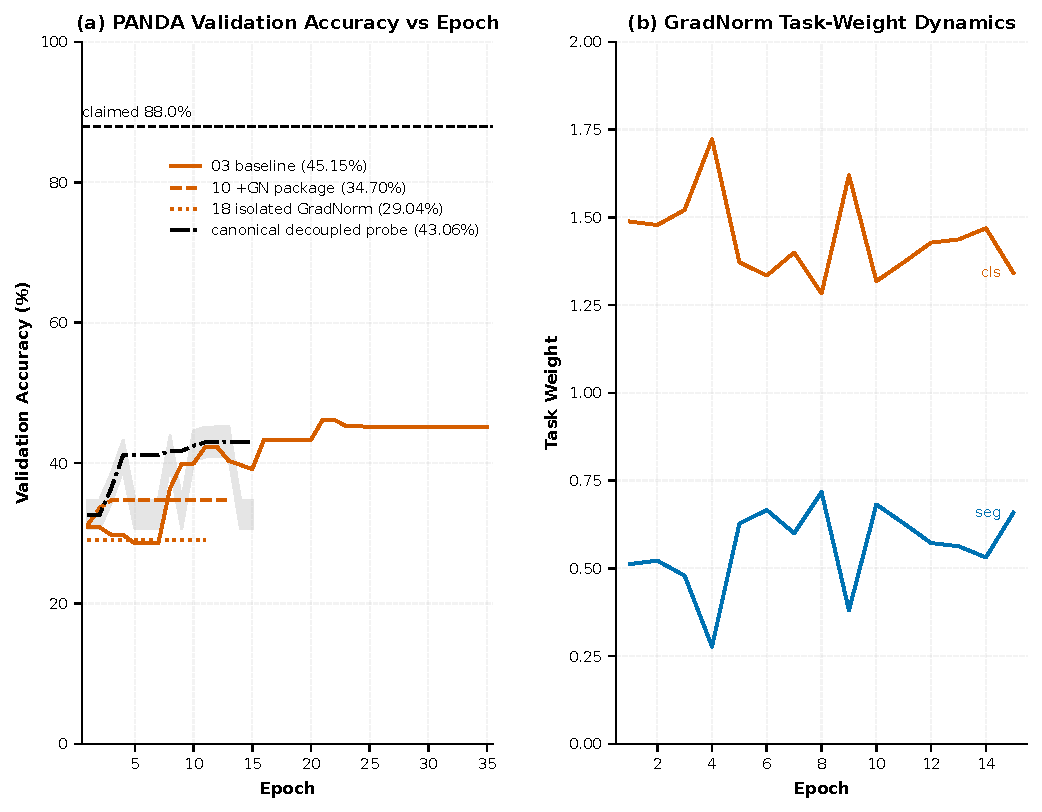
\includegraphics[width=\textwidth]{fig4_panda_anatomy.pdf}
\caption{Anatomy of the PANDA accuracy drop. (a) Validation accuracy vs.\ epoch (fold 1 of 5) for three PANDA runs --- Run 03 (static $5{:}1$ baseline), Run 10 (v2 GradNorm package), Run 18 (isolated GradNorm at $\eta=10^{-3}$) --- with legend values giving each run's five-fold mean accuracy ($34.51\%$, $37.56\%$, $28.21\%$); the canonical decoupled \textsc{GradNorm} arm is overlaid (dash-dot, fold-1 trajectory), with its five-fold mean $22.70\%$ (horizontal line) and 95\% bootstrap CI $[14.66, 30.73]$ (shaded band) marked --- $\approx 65.3$ percentage points below the claimed $88.0\%$ (black dashed reference). (b) \textsc{GradNorm} task-weight dynamics as recorded by the dedicated canonical optimizer probe (15 epochs; per-epoch weights are logged only by that probe): the segmentation weight collapses while the classification weight grows, showing the dynamic rebalancing that the joint variant turns into destructive updates on the shared encoder.}
\label{fig:panda_anatomy}
\end{figure}

\subsection{Controlled Skip Connection Ablation: A Verified Null Result}\label{sec:skip}
We evaluate skip connections in matched pairs, holding learning rate, GradNorm, and Macenko normalization identical:
\begin{itemize}
    \item \textbf{Coarse macro-tumor structures (TCGA):} Run 25 (skip-ablated) vs.\ matched baseline Run 08 (both $\eta=10^{-4}$, GradNorm, Macenko): accuracy $95.28\%$ vs.\ $95.26\%$ ($\Delta_{\text{Acc}} = +0.02$), Dice $86.16\%$ vs $89.22\%$ ($\Delta_{\text{Dice}} = -3.06$).
    \item \textbf{Fine micro-glandular structures (PANDA):} Run 26 (skip-ablated, $37.44\%$ Acc / $84.29\%$ Dice) vs.\ matched baseline Run 10 ($37.56\%$ / $82.77\%$): $\Delta_{\text{Acc}} = -0.12$, $\Delta_{\text{Dice}} = +1.52$.
\end{itemize}
In both cases the differences are small, and the 95\% bootstrap CIs across the five folds overlap substantially (TCGA: $[94.14, 96.28]$ vs $[94.24, 96.39]$; PANDA: $[36.73, 37.99]$ vs $[37.20, 37.94]$). We therefore report these as \emph{verified null results}: the bottleneck-only representation suffices for both coarse macro-lesion and fine micro-glandular segmentation, and zeroing the skips produces no detectable penalty in a five-fold comparison.

\paragraph{Macenko stain-normalization ablation.}
The matched Macenko pair (Group 5, Runs 23--24) is the only ablation with a statistically resolvable classification shift. Omitting normalization raises PANDA top-1 accuracy by $+3.81$ (Run 23: $41.38\%$ vs.\ Run 10: $37.56\%$) and PanNuke accuracy by $+2.75$ (Run 24: $99.24\%$ vs.\ Run 16: $96.49\%$) with disjoint 95\% bootstrap CIs across the five folds ($[39.76, 43.38]$ vs $[37.20, 37.94]$; $[99.11, 99.37]$ vs $[96.18, 96.90]$), while Dice rises modestly on PANDA ($84.39\%$ vs.\ $82.77\%$, $\Delta=+1.62$) and by $+8.51$ on PanNuke ($70.76\%$ vs.\ $62.25\%$). Color deconvolution thus harms fine-grained classification --- consistent with over-smoothing of the chromatin/texture cues on which grading relies --- and partially decomposes the v1-vs-v2 PANDA gap of \S\ref{sec:panda}. Figure~\ref{fig:ablation_forest} consolidates all six matched pairs; Figure~\ref{fig:macenko} shows the texture flattening.

\begin{figure}[!tbp]
\centering
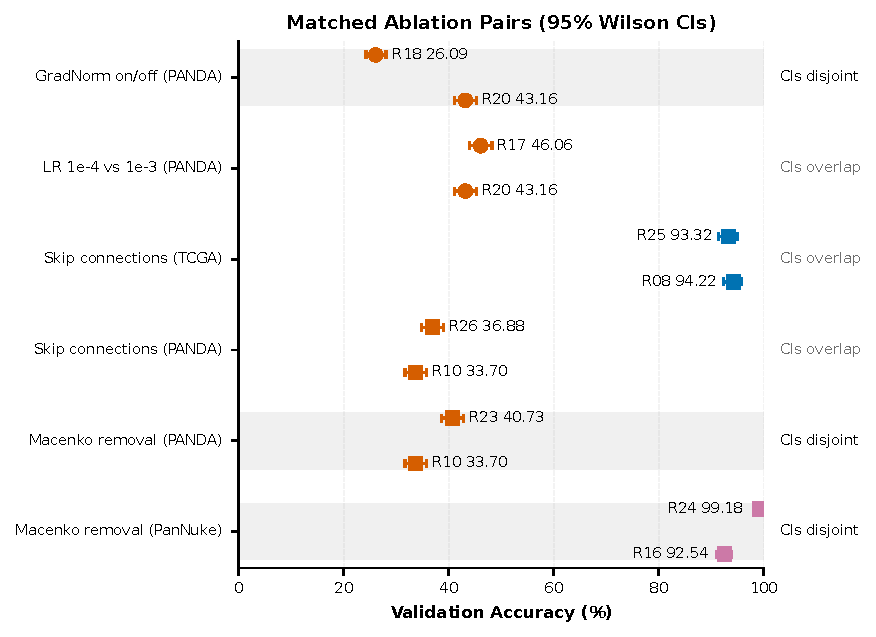
\includegraphics[width=\textwidth]{fig5_ablation_forest.pdf}
\caption{Matched-ablation forest plot of validation accuracy with 95\% bootstrap CIs across the five folds for the six strictly matched pairs. Disjoint-CI pairs (shaded): isolated GradNorm (Run 18, $28.21\%$) vs.\ static $5{:}1$ (Run 20, $38.18\%$); LR $10^{-4}$ vs.\ $10^{-3}$ (Runs 17 vs.\ 20: $44.87\%$ vs.\ $38.18\%$); no-Macenko PANDA (Run 23, $41.38\%$) vs.\ matched (Run 10, $37.56\%$); no-Macenko PanNuke (Run 24, $99.24\%$) vs.\ matched (Run 16, $96.49\%$). Overlapping-CI pairs: skip ablation TCGA (Runs 25 vs.\ 08: $95.28\%$ vs.\ $95.26\%$); skip ablation PANDA (Runs 26 vs.\ 10: $37.44\%$ vs.\ $37.56\%$). The right-margin verdict column encodes the CI-overlap test, so the null-result status of the skip ablations and the resolvable LR, Macenko, and GradNorm effects are read directly from the plot.}
\label{fig:ablation_forest}
\end{figure}

\subsection{Isolating Learning Rate from Dynamic Gradient Balancing}\label{sec:gn}
Group 4 (PANDA $\times$ VGG16) factorizes the key optimization hyperparameters: learning rate ($\eta \in \{10^{-3}, 10^{-4}\}$), GradNorm-style balancing (on/off), and static loss-weighting ratios $\lambda_{seg}:\lambda_{cls} \in \{1{:}10, 1{:}1, 5{:}1, 10{:}1\}$, all under raw inputs.

\paragraph{Direct Isolation of Dynamic Gradient Balancing (Run 18).}
The isolated GradNorm arm at $\eta=10^{-3}$ under matched raw-input conditions (Run 18: PANDA $\times$ VGG16, GradNorm $\alpha=1.5$, raw input) compares directly against the static 5:1 baseline (Run 20). Activating GradNorm ($\alpha=1.5$) collapses validation accuracy from $38.18\%$ to $28.21\%$ (95\% bootstrap CI across the five folds: $[24.76, 31.47]$) with non-overlapping confidence intervals ($[32.75, 41.79]$ vs $[24.76, 31.47]$, $\Delta_{\text{Acc}} = -9.97\%$), while Dice remains flat at $84.39\%$.

This $28.21\%$ accuracy matches the low-accuracy regime observed in Phase v2 at $\eta=10^{-4}$ (Run 09: $33.34\%$ Acc). The $\approx 22.7\%-33.4\%$ floor on 6-class PANDA grading under GradNorm is thus driven primarily by the $\alpha=1.5$ balancing formulation, whose gradient-norm equalization forces destructive updates onto the shared encoder.

\paragraph{Learning Rate and Loss Weighting Dynamics.}
Holding GradNorm off, reducing the learning rate from $\eta=10^{-3}$ (Run 20: $38.18\%$ Acc) to $\eta=10^{-4}$ (Run 17: $44.87\%$) yields a statistically resolvable improvement, with disjoint 95\% bootstrap CIs across the five folds. The static loss-ratio sweep (Runs 19--22) confirms $\lambda=5{:}1$ and $10{:}1$ as comparable static balances ($36.51\%$--$39.71\%$), yet no ratio approaches the claimed $87\%-88\%$ (Figure~\ref{fig:lambda_sweep}). The isolated GradNorm arm (Run 18) drops to $28.21\%$ against the $38.18\%$ static baseline with non-overlapping CIs, and the canonical decoupled scheme plateaus at $22.70\%$ (95\% bootstrap CI $[14.66, 30.73]$). Dynamic balancing in either formulation cannot bridge the gap (Figures~\ref{fig:panda_anatomy}, \ref{fig:ablation_forest}).

\begin{figure}[!tbp]
\centering
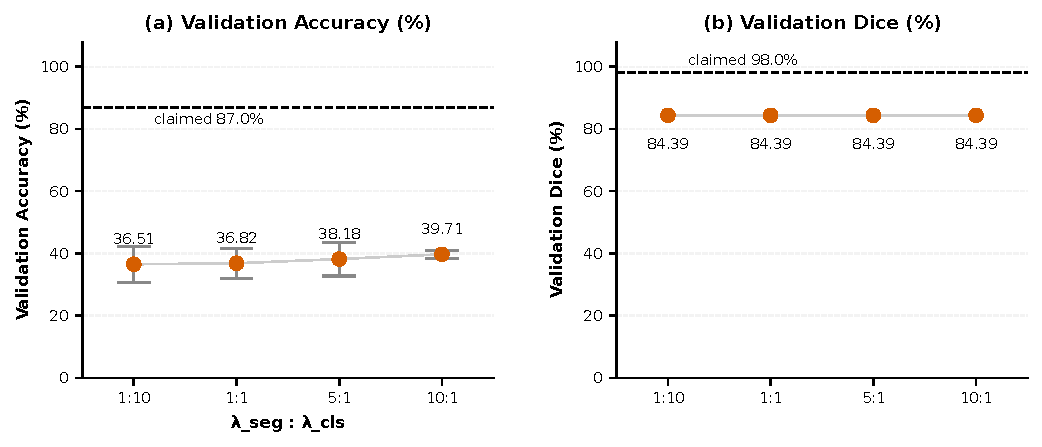
\includegraphics[width=\textwidth]{fig6_lambda_sweep.pdf}
\caption{Static loss-weight ratio sweep on PANDA $\times$ VGG16 (raw input, $\eta=10^{-3}$, no GradNorm). (a) Validation accuracy with 95\% bootstrap-CI whiskers across the five folds: $\lambda_{seg}:\lambda_{cls} = 1{:}10$ ($36.51\%$), $1{:}1$ ($36.82\%$), $5{:}1$ ($38.18\%$), $10{:}1$ ($39.71\%$); the black dashed line marks the claimed $87.0\%$ accuracy. (b) Validation Dice for the same four arms ($84.39\%$, $84.39\%$, $84.39\%$, $84.39\%$) against the claimed $98.0\%$. The ratios yield comparable accuracy ($36.51\%-39.71\%$), yet no ratio approaches the claimed target --- the gap is not a loss-weighting artifact.}
\label{fig:lambda_sweep}
\end{figure}

\section{Conclusion \& Recommendations}
Across 27 configurations $\times$ 5 folds (135 fold-cells), the claimed $88\%-99\%$ metrics did not reproduce under group-aware isolation (patient-level for TCGA, image/biopsy-level for PANDA, image-level for PanNuke, and a degenerate stratified 5-fold for SIIM, whose release has one image per patient). The residual gap stems from dataset difficulty and the joint optimization recipe: skip connections are a null result, while joint balancing ($\alpha=1.5$) destabilizes classification ($38.18\% \to 28.21\%$ Acc). We therefore recommend: (1) mandatory group-aware \texttt{GroupKFold} splitting at the finest grouping the release supports (patient, image/biopsy, or image), with the grouping unit and its cardinality reported explicitly; (2) explicit reporting of the Dice evaluation convention, with foreground-only or zero-penalty scoring on sparse-lesion datasets; (3) 95\% bootstrap CIs across the five folds on matched ablation comparisons, to distinguish genuine architectural effects from fold-to-fold variance; (4) validation on diverse multi-organ benchmarks such as PanNuke; and (5) systematic evaluation of multi-task balancing hyperparameters before clinical translation.

None of the mechanisms quantified here is exotic. Each is documented independently in the evaluation literature (Section~\ref{sec:related}), and the study whose figures motivated this audit is already being cited as evidence of multi-task efficacy in follow-on oncology work. The recommendations above are therefore offered not as a verdict on a single pipeline but as a minimum verification checklist for any joint detection--segmentation claim intended for clinical consumption.

\section*{Declaration of generative AI and AI-assisted technologies in the writing process}
AI-assisted tools were used for language refinement and figure preparation. All scientific content, experiments, data analysis, and conclusions are the sole work of the authors, who reviewed and approved the final manuscript.

\section*{CRediT author statement}
Muhammad Abdullah Ali: Conceptualization, Methodology, Software, Validation, Formal analysis, Investigation, Data curation, Visualization, Writing -- original draft, Project administration. Muhammad Ibrahim Kiani: Writing -- review \& editing. Muhammad Abdullah Aamir: Writing -- review \& editing.

\section*{Declaration of competing interest}
The authors declare that they have no known competing financial interests or personal relationships that could have appeared to influence the work reported in this paper.

\section*{Funding}
This research did not receive any specific grant from funding agencies in the public, commercial, or not-for-profit sectors.

\section*{Data availability}
All training scripts, per-run JSON summaries, evaluation checkpoints, generated figures, and the complete results matrix with 95\% Wilson score intervals~\cite{wilson1998score} (\texttt{paper\_results\_matrix\_with\_ci.csv}) are publicly available at \url{https://github.com/ApatheticMioz/cancer-pathology-dl}.

\bibliographystyle{elsarticle-num}
\bibliography{references}

\end{document}
